\documentclass[DynamicalBook]{subfiles}
\begin{document}
%


\setcounter{chapter}{0}%Just finished 0.


%------------ Chapter ------------%
\chapter{}


Here's a basic fact of life: \emph{things change}. And how things change most
often depends on how they currently are. This is the basic idea underlying all the various notions of \emph{dynamical
  system} that we will see in this book.

\begin{definition}
  A \emph{dynamical system} consists of:
  \begin{itemize}
  \item a notion of how things are, called the \emph{state}, and
  \item a notion of how things will change given how they are, called the \emph{dynamics}.
  \end{itemize}
  The dynamics of a system might also depend on some free \emph{parameters}, and
  we will often only be interested in some particular \emph{variables} of the
  state. 
\end{definition}

In this chapter, we will see this idea in its
most distilled form: we will know exactly how things are, and what they will be
like next. That is, we'll be focusing on \emph{deterministic} dynamical systems,
whose time steps forward in \emph{discrete} increments.

A paradigmatic example of this sort of dynamical system is a clock.
\[
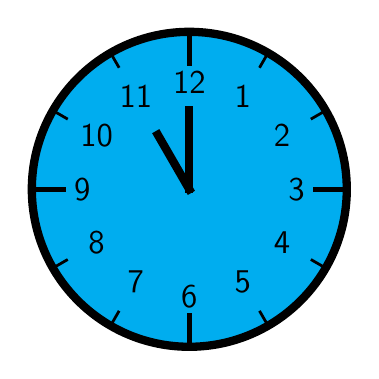
\begin{tikzpicture}[line cap=rect,line width=3pt]
\filldraw [fill=cyan] (0,0) circle [radius=2cm];
\foreach \angle [count=\xi] in {60,30,...,-270}
{
  \draw[line width=1pt] (\angle:1.8cm) -- (\angle:2cm);
  \node[font=\large] at (\angle:1.36cm) {\textsf{\xi}};
}
\foreach \angle in {0,90,180,270}
  \draw[line width=2pt] (\angle:1.6cm) -- (\angle:2cm);
\draw (0,0) -- (120:0.8cm);
\draw (0,0) -- (90:1cm);
\end{tikzpicture}
\]

Suppose that our clock has just an hour hand for now. Then we may collect all
the way things can be for the clock into a set of hours:
$$\Set{Hours} := \{1, 2, 3, 4, 5, 6, 7, 8, 9, 10, 11, 12\}.$$

The set $\Set{Hours}$ is the set of \emph{states} of our clock system. If we know what hour it is, we also know what hour is coming next. So, this system has the following dynamics:
\begin{align*}
  \fun{tick} &: \Set{Hours} \to \Set{Hours} \\
                i \mapsto \begin{cases} i + 1 &\mbox{if $i < 12$}\\ 1 &\mbox{if $i = 12$}  \end{cases}
\end{align*}

Here's a sample of the dynamics of the clock. Say we started at 3 o'clock:
$$3 \xmapsto{\fun{tick}} 4 \xmapsto{\fun{tick}} 5 \xmapsto{\fun{tick}} 6
\xmapsto{\fun{tick}} \cdots$$

Not the most dynamic of systems, but we have to start somewhere. If we want to
refer to the whole system at once, we can box it up and write it like this:

\begin{equation}\label{}\tag{box1}
\begin{tikzpicture}[oriented WD, bbx = 1cm, bby =.5cm, bb min width=1cm, bb port length=4pt, bb port sep=1]
	\node[bb={1}{1}] (X) {$M$};
	\draw[label] 
		node [left=2pt of X_in1] {$A$}
		node [right=2pt of X_out1] {$B$}
		;
\end{tikzpicture}
\end{equation}

\end{document}
